\chapter{Экспериментальные результаты}\label{ch:ch4}

\section{Апробация ПАЗЛ-3D для исследования алюминиевого сплава системы Al-Mg-Si}\label{sec:ch4/sect1}

После сборки и запуска ПАЗЛ-3D появилась необходимость по демонстрации возможностей установки по исследованию сплавов на основе алюминия  с наноразмерными особенностями. При этом материал должен был удовлетворять следующим требованиям. Материал - многокомпонентный сплав, имеющий хорошую теплопроводность. В нём должны присутствовать структуры с характерным размером от 10 до 100 нм. Вышеуказанные требования позволили, с одной стороны, продемонстрировать возможности установки по характеризации наноструктур и масс-спектрометрии, с другой стороны, материал позволяет максимально упростить проведение исследования, благодаря хорошей теплопроводности и электрической проводимости. Перечисленным требованиям отвечал сплав Al-Mg-Sc. Алюминиевые сплавы, в зависимости от легирующих элементов, могут обладать повышенной прочностью, пластичностью, коррозийной стойкостью, жаростойкость. Благодаря своим свойствам такие сплавы широко применяются как конструкционные материалы.

Для исследования выбранного сплава были выбраны следующие параметры исследования: температура образца 50К, мощность лазерного излучения с гармоникой 515 нм составляла 10 мВт, скорость сбора данных в ходе эксперимента лежала в пределах от 100 до 500 атомов/сек. Выбранные параметры являются наиболее часто используемые для исследования алюминиевых сплавов.

В результате проведения атомно-зондового исследования сплава были получены масс-спектр и атомные карты распределения элементов в образце. На Рисунке \cref{fig:AlMgSi_mass} представлена основная часть масс-спектра. Среднее разрешение по массе на полувысоте пика составило 500 единиц.

\begin{figure}[htb]
	\centerfloat{
		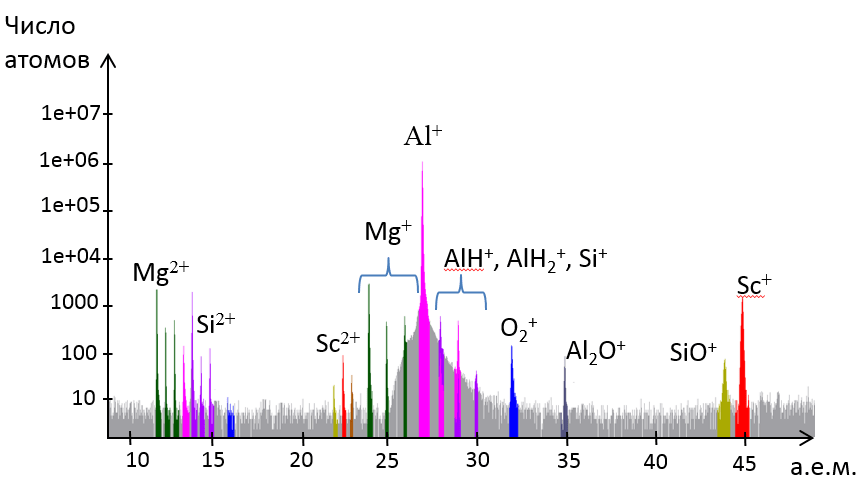
\includegraphics[width=.8\textwidth]{AlMgSi_mass}
	}
	\caption{Основная часть масс-спектра сплава Al-Mg-Sc.}
	\label{fig:AlMgSi_mass}
\end{figure} 
\FloatBarrier
Были обнаружены наноразмерные включения, обогащенные по элементам Mg, Si, O и Cu. На Рисунке \cref{fig:AlMgSi_3D} представлены изоповерхности (поверхности одинаковой концентрации) по магнию и кремнию с обогащением в 16$\%$ и атомные карты распределения магния и кремния.

\begin{figure}[htbp]
	\begin{minipage}[b][][b]{0.49\textwidth}\centering
		%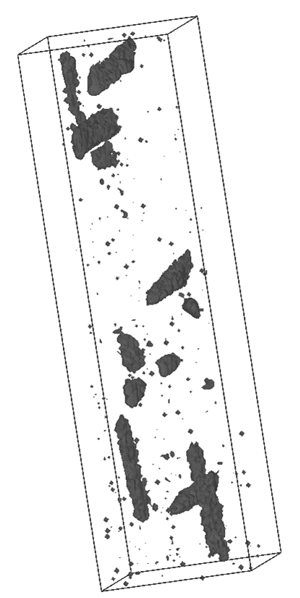
\includegraphics[width=\textwidth]{AlMgSi_3D_a} \\ а)
		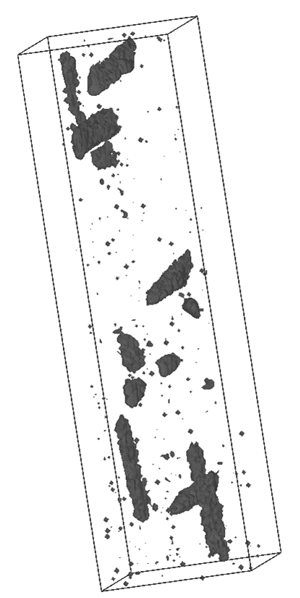
\includegraphics[scale=0.8]{AlMgSi_3D_a} \\ а)
	\end{minipage}
	%\hfill
	\begin{minipage}[b][][b]{0.49\textwidth}\centering
		%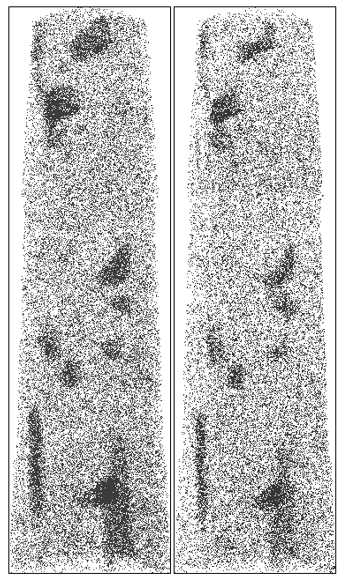
\includegraphics[width=\textwidth]{AlMgSi_3D_b} \\ б)
		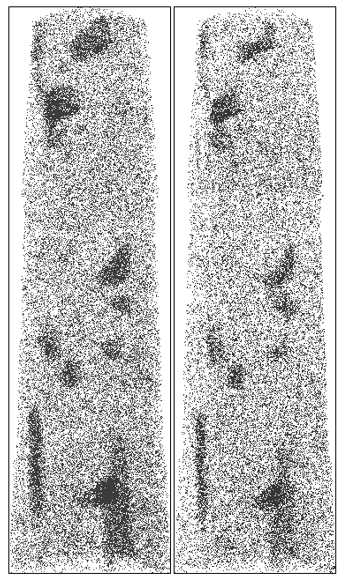
\includegraphics[scale=0.8]{AlMgSi_3D_b} \\ б)
	\end{minipage}
	\caption{а) Изоповерхность обогащения Mg и Si на 16$\%$ по сравнению с матрицей, б) атомные карты распределения магния (левый объем) и кремния (правый объем). Размер исследованной области 47х47х167 нм$^3$}
	\label{fig:AlMgSi_3D}
\end{figure} 

Обнаруженные включения имеют характерную длину порядка 50$\pm$10 нм и 10$\pm$2 нм в ширину. Размеры включений определялись по линейным размерам изоконцентрационных поверхностей. Объемная плотность составляет 2х$10^{22}$ см$^{-3}$. Ввиду несферической формы включений распределение по размерам не представляется возможным построить. Химический состав матрицы и включений показан в Таблице \cref{tab:AlMgSi_table}.

\begin{table} [htbp]
	\centering
	%\begin{threeparttable}% выравнивание подписи по границам таблицы
		\caption{Состав матрицы и включений сплава Al-Mg-Sc at. $\%$}%
		\label{tab:AlMgSi_table}%
		\begin{SingleSpace}
			\begin{tabular}{| c | c | c | c | c | c | c | c |}
				\hline
				  			& Al      & Mg     & Si    & Sc     & O     & Cu     \\ \hline
				Матрица     & 98.67   & 0.56   & 0.35  & 0.31   & 0.05  & 0.03   \\ \hline
				Включения   & 67.24   & 18.22  & 13.7  & 0.36   & 0.12  & 0.36   \\  \hline				
			\end{tabular}%
		\end{SingleSpace}
	%\end{threeparttable}
\end{table}

В данной работе продемонстрирована возможность исследования сплавов на основе алюминия на установке ПАЗЛ-3D. В качестве исследуемого материала выбран сплав Al-Mg-Sc. Получены масс-спектр образца и атомные карты распределения элементов. Обнаружены включения вытянутой формы. Рассчитана объемная плотность включений и химический состав матрицы и включений. Полученные результаты подтверждают широкие возможности установки ПАЗЛ-3D по возможностям проведения исследований.

\FloatBarrier

\section{Демонстрация возможности АЗТ по исследованию структуры среднеуглеродистой стали}\label{sec:ch4/sect2}

Для демонстрации возможностей АЗТ по исследованию среднеуглеродистых сталей были проведены исследования материала стали (C 0.45, Si 0.36, Mn 1.13, Ni 0.67, Cu 0.63, Cr 1.26, Mo 0.40, Ti 0.03, V 0.06, Nb 0.02, Ca 0.03, B 0.003, S 0.008, P 0.005 масс.\%) листового проката после отпуска при различных температурах. Основной целью было показать распределение углерода и легирующих элементов в объеме. 

(Условия исследования?)

Полученные атомные карты показаны на Рисунке \cref{fig:SteelAtomMaps1}, общий объем полученных данных составляет 23x23x200 нм$^{3}$. В Таблице \cref{tab:SteelComposition150} показан состав общий образца, состав матрицы и состав выделенных областей 1 и 2 на атомных картах.

\begin{figure}[ht]
	\centerfloat{
		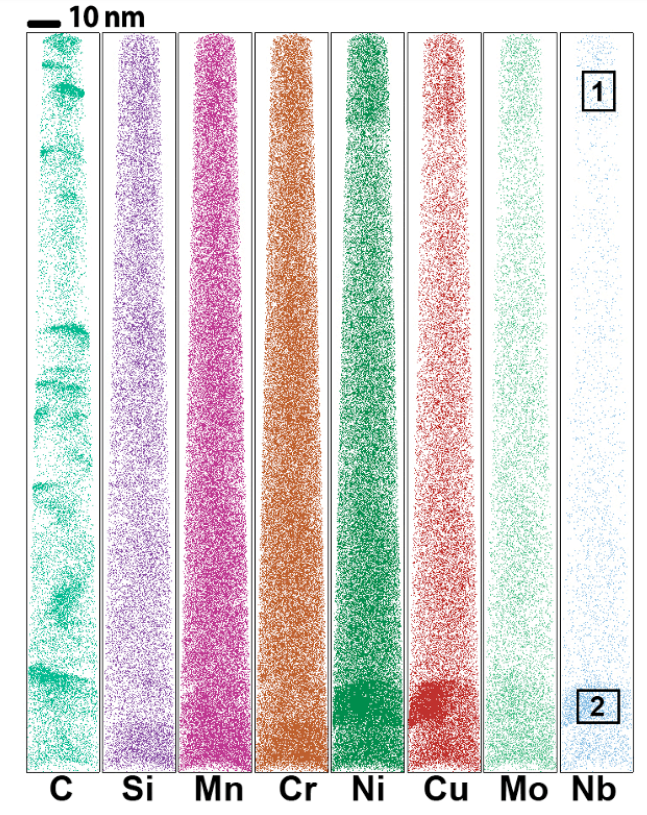
\includegraphics[width=.7\textwidth]{SteelAtomMaps1}
	}
	\caption{Атомные карты образца среднеуглеродистой стали после отпуска при 150 \textdegree С \cite{scbibRyabov}. Состав областей 1 и 2 показан в Таблице \cref{tab:SteelComposition150} }
	\label{fig:SteelAtomMaps1}
\end{figure} 

\begin{table} [htbp]
	\centering
	\caption{Состав образца, матрицы и областей 1 и 2 среднеуглеродистой стали после отпуска при температуре 150 \textdegree С (at.\%)}%
	\label{tab:SteelComposition150}%
	\begin{SingleSpace}
		\begin{tabular}{|p{3cm}| c | c | c | c | c | c | c | c | c | c | c |}
			\hline
			& C & Si & Mn & Ni & Cu & Cr & Mo & Ti & V & Nb & Al     \\ \hline
			For ladle sample     & 0.45 & 0.36 & 1.13 & 0.67 & 0.63 & 1.26 & 0.40 & 0.03 & 0.06 & 0.02 & 0.04   \\ \hline
			Среднее по объему   & 0.45 & 0.42 & 1.11 & 0.49 & 0.62 & 1.37 & 0.23 & - & 0.07 & 0.10 & 0.04   \\  \hline		
			Матрица   & 0.26 & 0.41 & 1.09 & 0.38 & 0.46 & 1.34 & 0.19 & - & 0.07 & 0.05 & 0.05   \\  \hline	
			Область 1   & 0.97 & 0.53 & 1.31 & 0.49 & 0.51 & 1.54 & 0.32 & - & 0.08 & 0.12 & 0.09   \\  \hline
			Область 2   & 0.71 & 0.28 & 1.12 & 0.94 & 1.05 & 1.34 & 0.38 & - & 0.07 & 0.32 & 0.04   \\  \hline	
		\end{tabular}%
	\end{SingleSpace}
\end{table}

Для анализа локального распределения элементов построен профиль линейных концентраций вдоль всего образца (Рисунок \cref{fig:SteelLinear1}). По линейным концентрациям и атомным картам можно явно определить наличие областей с повышенным содержанием углерода и оценить их морфологию и состав. Средняя концентрация углерода в углеродных включениях составляет 1.5 ат.\%. Присутствует также одна сегрегация углерода, обогащенная также никелем, ниобием и молибденом.

\begin{figure}[ht]
	\centerfloat{
		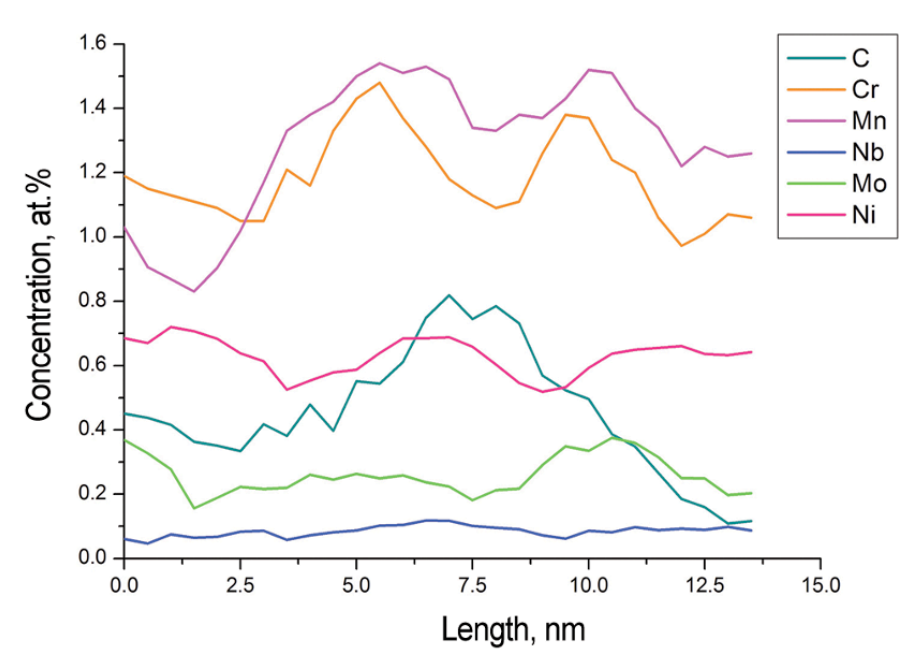
\includegraphics[width=.8\textwidth]{SteelLinear1}
	}
	\caption{Линейные профили концентраций для образца среднеуглеродистой стали после отпуска при 150 \textdegree С \cite{scbibRyabov}}
	\label{fig:SteelLinear1}
\end{figure}

\begin{figure}[htb]
	\centerfloat{
		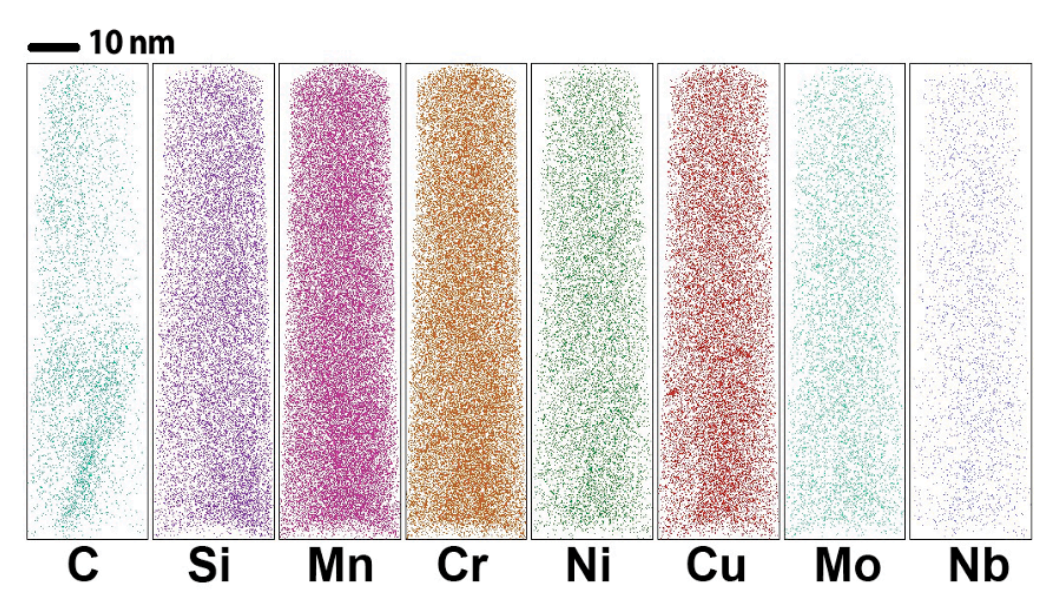
\includegraphics[width=.8\textwidth]{SteelAtomMaps2}
	}
	\caption{Атомные карты образца среднеуглеродистой стали после отпуска при 350 \textdegree С \cite{scbibRyabov}}
	\label{fig:SteelAtomMaps2}
\end{figure}

Для второго состояния материала после отпуска при 350 \textdegree С также получены атомные карты (Рисунок \cref{fig:SteelAtomMaps2}). Размер полученных данных составляет 25х25х100 нм$^{3}$. В Таблице \cref{tab:SteelComposition350} показан состав массивного образца и матрицы. Состав матрицы, без учета включений примерно соответствует составу массивного образца за исключением углерода, молибдена и ниобия. 

Для более детальной характериазции углеродного включения построен отдельный линейный профиль концентрации для малого 3D объема на Рисунке \cref{fig:SteelLinear2}. Данный профиль наглядно демонстрирует обогащение углеродом границы (зерна??) до 0.8 ат.\%, а также заметно обогащение по хрому и марганцу до 1.5ат.\% каждый.

\begin{figure}[htb]
	\centerfloat{
		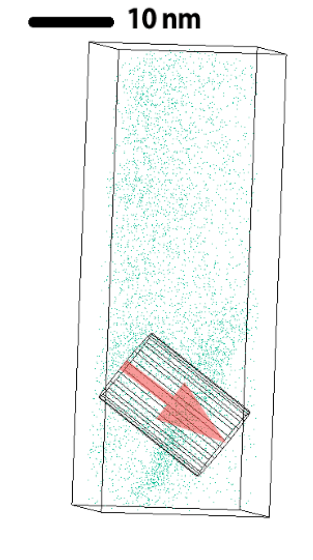
\includegraphics[width=.3\textwidth]{SteelAtomMapsLin}
	}
	\caption{Область построения линейной концентрации для границы (зерна?)\cite{scbibRyabov}}
	\label{fig:SteelAtomMapsLin}
\end{figure}

\begin{figure}[htb]
	\centerfloat{
		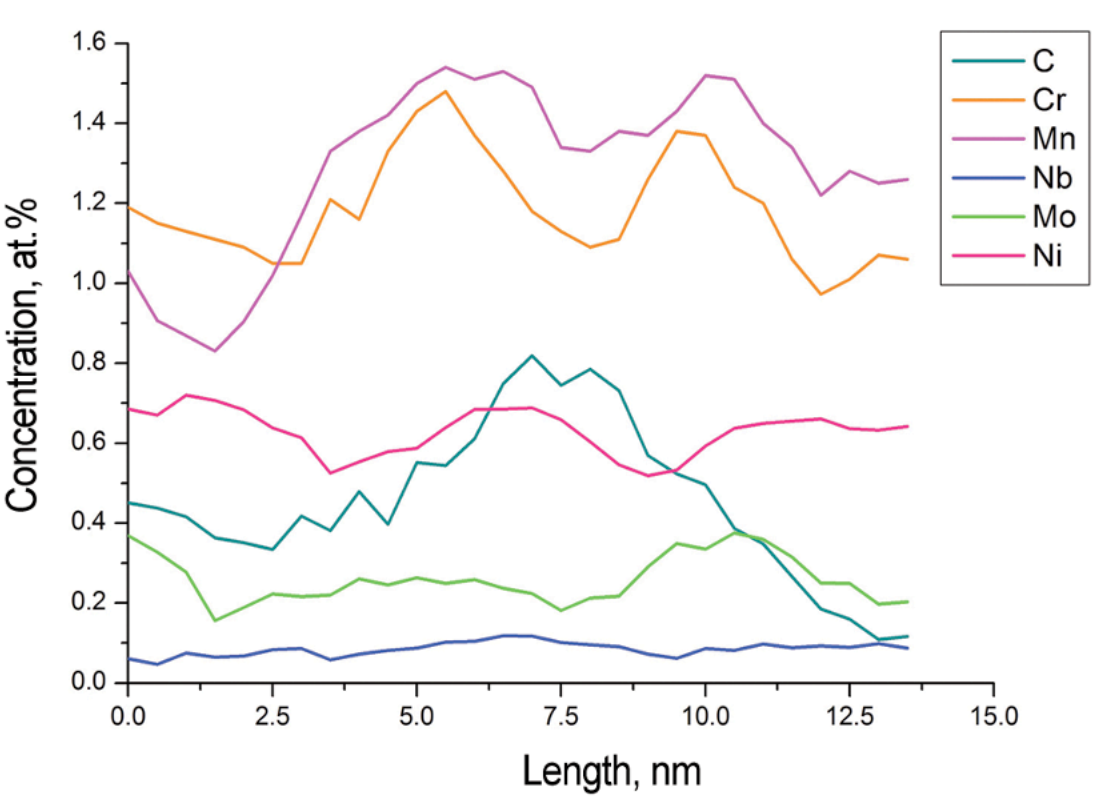
\includegraphics[width=.8\textwidth]{SteelLinear2}
	}
	\caption{Линейные профили концентраций для границы (зерна?) образца среднеуглеродистой стали после отпуска при 350 \textdegree С \cite{scbibRyabov}}
	\label{fig:SteelLinear2}
\end{figure}

\begin{table} [htbp]
	\centering
	\caption{Состав образца, матрицы и областей 1 и 2 среднеуглеродистой стали после отпуска при температуре 350 \textdegree С (at.\%)}%
	\label{tab:SteelComposition350}%
	\begin{SingleSpace}
		\begin{tabular}{|p{3cm}| c | c | c | c | c | c | c | c | c | c | c |}
			\hline
			& C & Si & Mn & Ni & Cu & Cr & Mo & Ti & V & Nb & Al     \\ \hline
			For ladle sample     & 0.45 & 0.36 & 1.13 & 0.67 & 0.63 & 1.26 & 0.40 & 0.03 & 0.06 & 0.02 & 0.04   \\ \hline
			Среднее по объему   & 0.37 & 0.41 & 1.16 & 0.61 & 0.57 & 1.37 & 0.23 & - & 0.07 & 0.10 & 0.05   \\  \hline		
			Матрица   & 0.37 & 0.40 & 1.14 & 0.60 & 0.55 & 1.35 & 0.22 & - & 0.07 & 0.10 & 0.05   \\  \hline		
		\end{tabular}%
	\end{SingleSpace}
\end{table}
\FloatBarrier
Исследования методом атомно-зондовой микроскопии позволили выявить многочисленные сегрегации атомов углерода в образце после отпуска при 150 \textdegree C. Полученные данные хорошо согласуются с данными просвечивающей электронной микроскопии: после отпуска при 150 \textdegree C наблюдались наиболее мелкие карбиды со средним размером 13 нм и объемной плотностью $220*10^{20} m^{-3}$. 
Для состояния  с большей температурой отпуска 300 \textdegree C наблюдаются крупные частицы размером до 164–180 нм на границах реечного мартенсита и на границах исходных аустенитных зерен, где остаточный аустенит с объемной долей встречается и до 5\%.

\FloatBarrier

\section{Исследование изменения структуры высокопрочной экономнолегированной стали}\label{sec:ch4/sect3}

Одной из актуальных задач в разработке низкоугеродистых сталей является повышение уровня прочности и требуемой прокаливаемости при закалке \cite{scbibGlubev}. Данный класс материалов важен в разработке новых атомных ледоколов и морских технических средств добычи углеводородов. Для улучшения основных характеристик материала используются различные системы легирования. В процессе закалки или высокотемпературного отпуска может изменяться как микро, так и наноструктура материала. Соответственно, атомно-зондовая томография может предоставлять важную информацию о локальном распределении химических элементов в данных материала на различных этапах обработки.

Для демонстрации возможности исследований данных сталей с помощью АЗТ был а использована сталь 09ХГН2МД. Состав стали мас. \%: 0.090 С; 30 Si; 0.70 Mn; 3.0 (Cr+Ni+Cu+Mo); 0.027 (V+Nb); 0.04 Al; 0.004 Ti; 0.002 Sn; 0.006 N; 0.003 S; 0.007 P. Образцы для исследования готовились стандартным способом: с помощью электроэрозионного станка и электро-химического утонения в 2-\%-ном растворе $HClO_{4}$ в бутоксиэтаноле. Были изучены три состояния,  состав образца и кластеров(при их наличии) показан в Таблице \cref{tab:SteelComposition09X}.

%\begin{itemize}
%	\item Закалка от 950 \textdegree C
%	\item Закалка от 950 \textdegree C + отпуск при 570 \textdegree С
%	\item Закалка от 950 \textdegree C + отпуск при 630 \textdegree С
%\end{itemize}

\begin{table} [htbp]
	\centering
	\caption{Состав образцов и кластеров для 09ХГН2МД (средние значения), ат.\%}
	\label{tab:SteelComposition09X}%
	\begin{SingleSpace}
		\begin{tabular}{| c | c | c | c | c | c | c | c | c |}
			\hline
			Состояние & & C & Si & Mn & Ni & Cr & Mo & Nb     \\ \hline
			For ladle sample     & 0.45 & 0.36 & 1.13 & 0.67 & 0.63 & 1.26 & 0.40 &    \\ \hline
			Среднее по объему   & 0.37 & 0.41 & 1.16 & 0.61 & 0.57 & 1.37 & 0.23 &   \\  \hline		
			Матрица   & 0.37 & 0.40 & 1.14 & 0.60 & 0.55 & 1.35 & 0.22 &   \\  \hline		
		\end{tabular}%
	\end{SingleSpace}
\end{table}

\FloatBarrier

\section{Исследование алюминия МИСиС Торгом}\label{sec:ch4/sect4}

Ожидает согласования с МИСиС Торгом

\FloatBarrier
\clearpage



%\nopagebreak - не разрывать страницами?







